\chapter{Detail design}\label{ch:detail_design}
%**********************************************
\section{System diagram}
\begin{figure}[H]
\centering
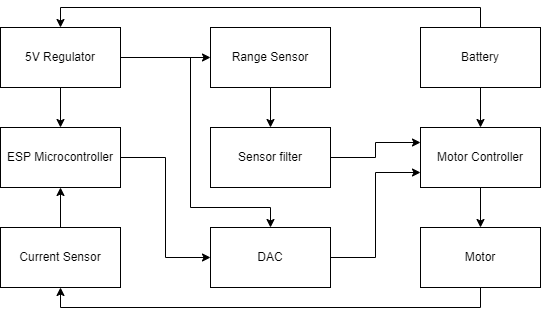
\includegraphics[width=0.9\linewidth]{./Figures/SystemDiagram.png}
\caption{System Diagram}
\label{fig:systdiag}
\end{figure}

\clearpage
\section{Current sensor}\label{sec:current_sensor_design}
The maximum operating current of the motor will be taken as \SI{300}{\milli\ampere}. With an $R_{sense}$ of \SI{10}{\milli\ohm} resulting in a max output voltage of \SI{3}{\milli\volt}. Since the op amp output will clip at \SI{5}{\volt} a gain of 1666 is required to have the output reach its max at the operating limit.\\

In order to filter out noise at the signal input a first order filter will be used. With the gain stated above the filtering will need to be quite hard to reduce noise at \SI{1}{\kilo\hertz} with an amplitude of \SI{10}{\milli\volt} to less than \SI{250}{\milli\volt} at the output. The following calculation was used to determine the cutoff frequency: 

\begin{align*}
Attenuation_{DB} & = 20 log \left( \frac{V_{noise-out(max)}}{V_{noise-in(max)} \cdot Gain} \right) \\
\omega_{cutoff} & = \frac{-Attenuation_{DB}}{-20} + log(\omega_{noise})\\
f_{cutoff} & = \frac{10^{\omega_{cutoff}}}{2 \pi}
\end{align*}
The above calculations result in a cutoff frequency of \SI{15}{\hertz}.The cutoff frequency and the response time of the circuit are inversely proportional. With the calculated cutoff frequency the response time of the circuit will be approximately \SI{70}{\milli\second} which meets the requirements. The noise on the output will be very close to \SI{250}{\milli\volt} with this cutoff frequency however a voltage divider will be placed on the output of the op amp in order to reduce the voltage to a \SI{3.3}{\volt} maximum. This will also reduce the noise amplitude to meet the specifications.\\

Figure: \ref{fig:cursen_sim_cir} shows the circuit configuration for the design mentioned above. To reach the required gain $R_3$ was chosen to be \SI{3330}{\ohm} therefore $R_2$ must be \SI{560}{\kilo\ohm}. $C_1$ was chosen to be \SI{100}{\nano\farad}, using the cutoff frequency calculated above $R_4$ must be \SI{100}{\kilo\ohm}. The voltage divider must have a high resistance in order to not load the opamp to heavily so values of \SI{33}{\kilo\ohm} and \SI{66}{\kilo\ohm} were chosen for $R_4$ and $R_5$.

\begin{figure}[H]
\centering
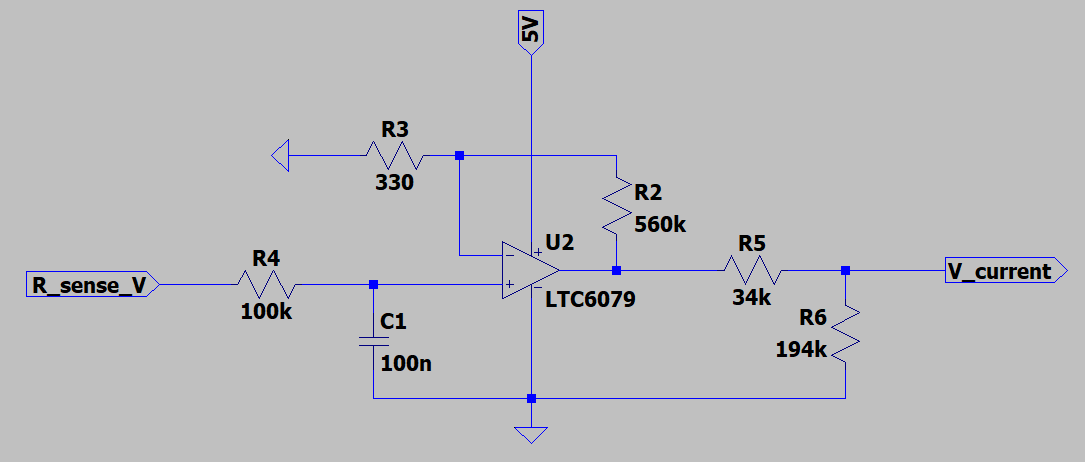
\includegraphics[width=0.65\linewidth]{./Figures/CurSens_SimCir.png}
\caption{Current sensing circuit design}
\label{fig:cursen_sim_cir}
\end{figure}

\newpage
\section{Analogue range sensor}
The HC-SR04 ultrasonic sensor requires a \SI{5}{\volt} supply and requires \SI{15}{\milli\ampere} to operate \cite{Design_SonicSens}. The frequency of the sensor output is the same as the input trigger frequency which is \SI{16}{\hertz}. Using a maximum distance of \SI{1}{\meter} and a minimum distance of \SI{5}{\centi\meter} results in a minimum duty cycle of 0.4\% and a maximum duty cycle of 10\%. The output pulses will have a maximum amplitude of  \cite{Design_SonicSens}.

Equation \ref{eqn:sens_gain} is used to calculate the needed gain of the system. In order to have the gain stage output a maximum of \SI{5}{\volt} at \SI{1}{\meter} a gain of 10.77 is required.

\begin{align}
Gain &= \frac{V_{Expected}}{V_{Duty Cycle \cdot V_{Amplitude}}}\label{eqn:sens_gain}
\end{align}

In order to determine the corner frequency fist the minimum attenuation must be calculated. The minimum attenuation can be calculated using the gain and amplitude of the first harmonic frequency component in the square wave to determine the size of the output ripple voltage, see Equation \ref{eqn:sens_harm}. Since the second harmonic and higher will all be attenuated more aggressively than the first harmonic it will contribute the most to the ripple voltage. 

\begin{align}
First Harmonic Amplitude &= V_{Amplitude} \cdot DutyCycle \cdot sinc(\pi \cdot DutyCycle)\label{eqn:sens_harm}\\
MinimumAttenuation &= 20log(\frac{MaximumNoise}{FirstHarmonicAmplitude \cdot Gain})\label{eqn:sens_atten}
\end{align}

Using Equation \ref{eqn:sens_atten} it is determined that an attenuation of atleast \SI{-41}{\decibel} is needed at \SI{16}{\hertz}. The corner frequency is then determined solving a simple straight line graph equation as shown in Equation \ref{eqn:sens_cutoff}.

\begin{align}
log(w) &= \frac{MinimumAttenuation+AttenuationSlope \cdot log(2\pi \cdot F_{trigger})}{AttenuationSlope}\\
F_{cutoff} &= 10^{2\pi \cdot log(w)}\label{eqn:sens_cutoff}
\end{align}

To determine what order filter to use Equation \ref{eqn:sens_cutoff} was solved using the different gradients for 1st, 2nd and 3rd order filters. Table \ref{tbl:sens_cutoff} shows the results of these calculations. In order to adhere to the response time specifications of \SI{1.5}{\second} it was decided that a 3rd order filter would have the best response time and noise attenuation without being to complex to build. 

\begin{table}
\begin{center}
\begin{tabular}{|c|c|c|}
\hline
Filter & Gradient & Maximum corner frequency\\
\hline
1st & \SI{-20}{\decibel} & \SI{0.13}{\hertz}\\
2nd & \SI{-40}{\decibel} & \SI{1.44}{\hertz}\\
3rd & \SI{-60}{\decibel} & \SI{3.2}{\hertz}\\
\hline
\end{tabular}
\end{center}
\caption{Filters and their maximum required corner frequency}
\label{tbl:sens_cutoff}
\end{table}

Design document \cite{Design_SonicSens_Filter} was used in the design of the 3rd order filter. Figure: \ref{fig:sonicsens_filter} shows the filter configuration that will be used. A simple gain stage will be appended to the end of the filter and then a voltage divider will ensure that the final output voltage is less than \SI{3.3}{\volt}. The whole circuit diagram is shown in Figure: \ref{fig:sonicsens_diag}. The circuit is designed to take input with an amplitude of \SI{5}{\volt} with a duty cycle between 0\% and 10\%.

The design document gives nominal values of R1=\SI{1.6}{\kilo\ohm} R2=\SI{2.4}{\kilo\ohm}  R3=\SI{7.5}{\kilo\ohm} C1=\SI{100}{\nano\farad} C2=\SI{10}{\nano\farad} C3=\SI{47}{\nano\farad} to construct a third order filter with a  corner frequency of \SI{1}{\kilo\hertz}. It was decided to design for a corner frequency of \SI{2}{\hertz} as this provides a good compromise between noise reduction and response time. In order to achieve this corner frequency frequency and impedance scaling was used on the given component values to get them to acceptable values that are easy to implement and result in minimal current draw. 


For the gain stage resistors R5 = \SI{22}{\kilo\ohm} and R6 = \SI{220}{\kilo\ohm} potentiometer. This will allow for a gain of up to 10 as calculated, however as shown in Figure: \ref{fig:sonicsens_diag} a lower gain is required to achieve the desired circuit response. This is due to practicalities such as rise time increasing the DC component of the input signal.


The voltage divider, R7 and R8 in Figure: \ref{fig:sonicsens_diag}, is to reduce the maximum output of \SI{5}{\volt} from the gain stage to a maximum of \SI{3.3}{\volt} to be used as input to the micro-controller. The resistor values are chosen to reduce current draw.

\begin{figure}
\centering
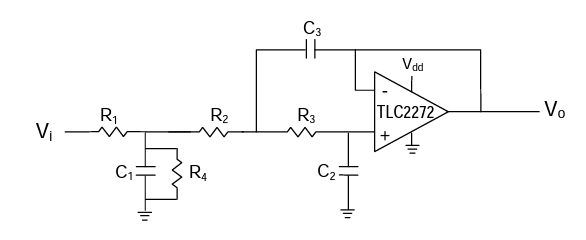
\includegraphics[width=0.5\textwidth]{./Figures/SonicSens_Filter.png}
\caption{Filter configuration from \cite{Design_SonicSens_Filter}}
\label{fig:sonicsens_filter}
\end{figure}

\begin{figure}
\centering
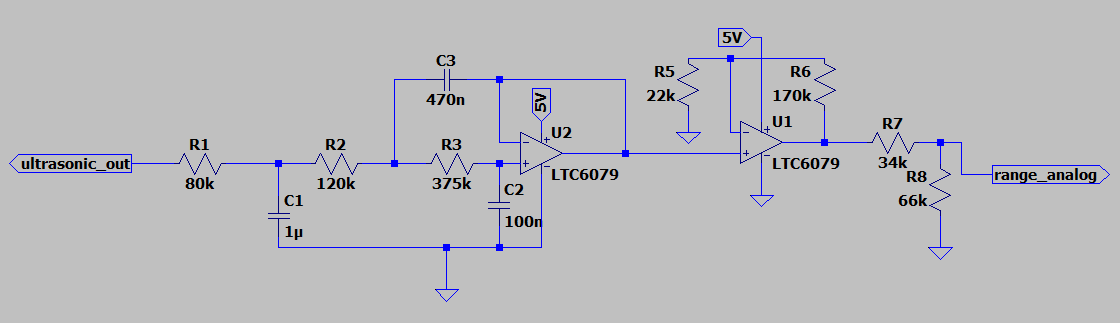
\includegraphics[width=0.9\textwidth]{./Figures/SonicSens_Diagram.png}
\caption{Filter configuration from \cite{Design_SonicSens_Filter}}
\label{fig:sonicsens_diag}
\end{figure}

\clearpage
\section{Digital to Analogue converter}
The input impedance seen by each source is equal to the resistor between it and the inverting input \cite{Lit_SumAmp_ET}. Thus to reduce the effect of the output impedance of the source the smallest input resistor must be much larger than the output impedance.

The operation of the DAC is not affected by the input impedance of the receiving circuit unless the input impedance is so low as to cause the op amp to reach it's current limits of \SI{23}{\milli\ampere} \cite{Data_MCP}. This will result in the op amp being unable to drive the required output voltage and the output voltage will be limited. A buffer will be added between the DAC and the output, this separates the output from the input and prevents any signal reflections from making it back to the input terminals.
\medskip\\
The MCP6242 has a common mode voltage range of $V_{SS} -0.3 < V_{CMR} < V_{DD} +0.3$ \cite{Data_MCP}. For the configuration shown in \ref{fig:DAC_sim_sumAmp} the common mode voltage will be the offset voltage applied at the positive terminal. As long as this offset voltage is less than the rail voltage there will be no problems with the op amps common mode voltage restrictions.

The maximum expected input will be \SI{3.3}{\volt}. The maximum output is \SI{3.3}{\volt} however the configuration show in Figure: \ref{fig:DAC_sim_sumAmp} can output up to \SI{5}{\volt}, this can only happen if the input voltages go negative.

$R_{off}$ is chosen to be \SI{100}{\kilo\ohm} in order to reduce current draw and $R_{base}$ is chosen to be \SI{50}{\kilo\ohm} to ensure high input impedance. Equation: \ref{eqn:DAC_rfr1} shows the relationship between the base resistor and the feedback resistor base on the maximum desired output. Equation: \ref{eqn:DAC_voff} shows what $V_{off}$ will be based on the maximum desired output. 

Potentiometers will be used to control the offset voltage and gain of the op amp as theses values are critical to the correct operation of the circuit and will require tuning.

 %V_{Out} &= V_{off} \left[1+ \frac{R_f}{R_1} \cdot \left(1+\frac{1}{2} + \frac{1}{4} + \frac{1}{8} \right) \right] - \frac{R_f}{R_1} \left[ V_{b3} +\frac{V_{b2}}{2} + \frac{V_{b1}}{4} + \frac{V_{b0}}{8} \right]\\
 %V_{off} &= \frac{V_{OutMax}}{1+\frac{15 \cdot R_f}{8 \cdot R_1}}\\
 %0 &= V_{off}\left[1+\frac{15 \cdot R_f}{8 \cdot R_1}\right] - \frac{15 \cdot R_f}{8 \cdot R_1} \cdot V_{InMax}\\
\begin{align}
\frac{R_f}{R_1} &= \frac{8 \cdot V_{OutMax}}{15 \cdot V_{InMax}}\label{eqn:DAC_rfr1}\\
V_{off} &= \frac{V_{OutMax}}{1+\frac{V_{OutMax}}{V_{InMax}}}\label{eqn:DAC_voff}
\end{align}

\begin{figure}[H]
\centering
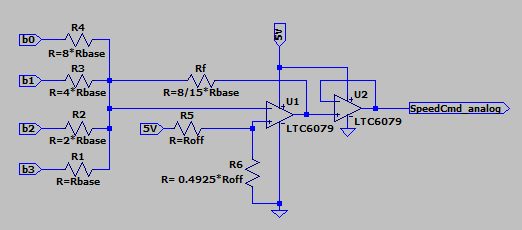
\includegraphics[width=0.5\textwidth]{./Figures/DAC_sim_cir.png}
\caption{Summing amplifier configuration}
\label{fig:DAC_sim_sumAmp}
\end{figure}

\clearpage
\section{Motor control signal}
The signal to control the motor speed must track the the input given by the micro controller but be limited by the input from the range sensor. A differential amplifier is perfect for this as it works as voltage subtractor. The configuration is shown in Figure: \ref{fig:mtrl_ctrl_dif}. 
In order to give equal weighting to each input $R_1 = R_2$ and $R_3 = R_4$. This results in $V_{OUT} = \frac{R_3}{R_1} (V_2-V_1)$. It was chosen for $R_1$ and $R_2$ to be \SI{56}{\kilo\ohm} and $R_3$ and $R_4$ will be potentiometers to allow for tuning of the gain. The desired gain will be $\frac{V_{bat}}{3.3}$\\

The max inputs will be \SI{3.3}{\volt} at each input which will result in a common mode voltage of < \SI{3.3}{\volt}. The max output of this control circuit must equal $V_{bat}$. Since the MCP6242 has max rail voltage of \SI{5.5}{\volt} a different op amp must be used. For this circuit the TLC2272 op amp will be used. This op amp can have up to \SI{8}{\volt} at it's positive rail and the maximum current draw is \SI{50}{\milli\ampere} \cite{TLC2272}.

\begin{figure}[H]
\centering
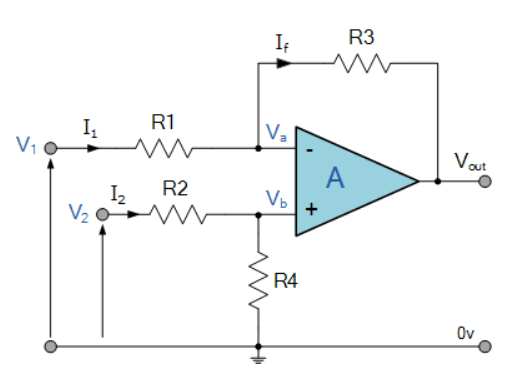
\includegraphics[width = 0.6\textwidth]{./Figures/Mtr_Ctrl_Dif.png}
\caption{Circuit diagram for a differential amplifier \cite{DifAmp}.}
\label{fig:mtrl_ctrl_dif}
\end{figure}

\clearpage
\section{Motor driver}
Since the motor requires a large amount of current in order to be driven the op amp can't drive the motor directly. Thus a current amplifier stage is required between the op amp and the motor. Since the current gain of the power transistor is relatively small, only using a single transistor will cause the op amp to supply more current.//

The op amp's ability to drive a voltage close to it's rail drops off sharply as the current draw increases \cite{TLC2272}. Thus a Darlington pair will significantly reduce the load placed on the op amp however this comes with the downside of reducing the maximum voltage that can be placed across the motor by the $V_{BE(on)}$ of the second transistor. With a Darlington pair made of a 2N2222 and a TIP31C as shown in Figure: \ref{fig:mtrctrl_darling} the max motor voltage is $V_{bat} - 1.4$.

\begin{figure}[H]
\centering
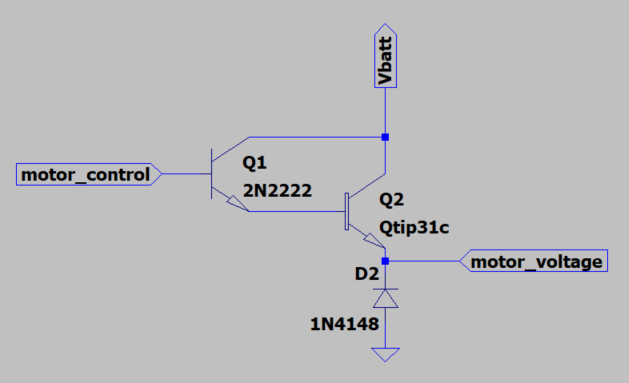
\includegraphics[width =0.5\textwidth]{./Figures/Mtr_Ctrl_Darling_Cir.png}
\caption{Darlington pair circuit configuration.}
\label{fig:mtrctrl_darling}
\end{figure} 

\clearpage
\section{Voltage regulation}
Using the configuration shown in Figure: \ref{fig:volt_reg_diag} the following equation determines the output voltage:
\begin{align*}
V_{OUT} &= V_{REF} \left(1+\frac{R_2}{R_1}\right)
\end{align*}

With a desired output voltage of \SI{5}{\volt} and a reference voltage of \SI{1.25}{\volt} results in a resistor ratio of $3R_1 = R_2$. So resistors of \SI{820}{\ohm} and \SI{270}{\ohm} are chosen to reduce complexity.

\begin{figure}[H]
\centering
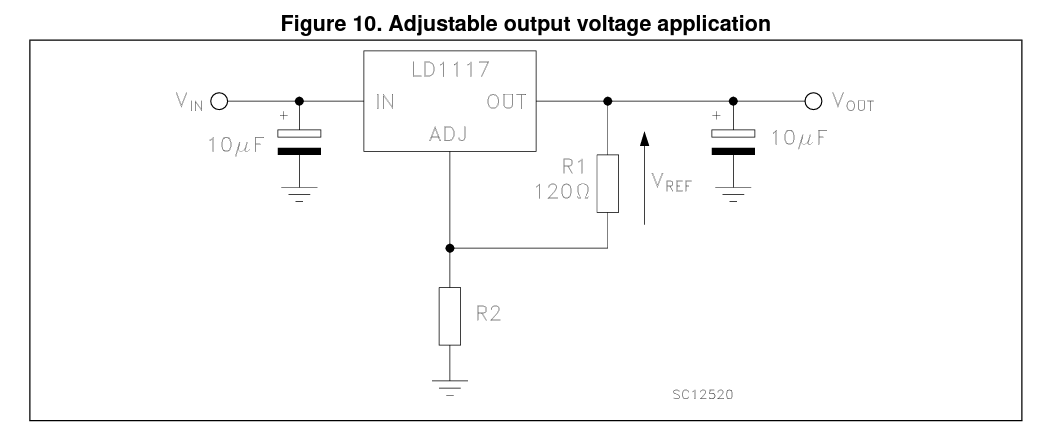
\includegraphics[width = 0.9\textwidth]{./Figures/Volt_Reg_Diag.png}
\caption{Circuit diagram used for the voltage regulator \cite{LD1117}.}
\label{fig:volt_reg_diag}
\end{figure}

\clearpage
\section{Low side switching circuit}

The low side switching circuit will be implemented with a nmos transistor. The following transistors are options to be used, however not all meet the required specifications of the circuit. The relevant electronic specifications for each transistor are shown in \ref{tbl:nmos}. The threshold gate voltage must be less than \SI{3.3}{\volt} as the circuit needs to be controlled by the ESP. The transistor must be able to take current up to \SI{1.5}{\ampere} as if the motor stalls the switching circuit mustn't break. The series resistance must be low otherwise the voltage across the motor will be too low. The only transistor that follows these requirements is the FQD13N06L.

A pull down resistor is required at the gate terminal of the nmos as if the board isn't driving the pin the gate will float and the motor will turn on. The resistor must be large enough not to load the ESP, thus a resistor of \SI{22}{\kilo\ohm} was chosen as this results in a current of \SI{150}{\micro\ampere}. The switching circuit can be seen in Figure:\ref{fig:low_switch_cir}.

In order to determine what frequency PWM control signal to use the cut-off frequency for the motor circuit must be determined. Using a frequency test the inductance of the motor was found to be \SI{1.5}{\milli\henry} and the resistance is \SI{5.4}{\ohm}.The equation $f = \frac{1}{2 \pi \frac{L}{R}}$ is used to calculate the cutoff frequency. With the stated values this results in a cutoff frequency of \SI{573}{\hertz}. However using frequencies below \SI{20}{\kilo\hertz} results in a tone audible to humans therefore it is decided to use a frequency of \SI{20}{\kilo\hertz} as this is well within the limits of the transistor.

\begin{table}[H]
\centering
\begin{tabular}{|l|l|l|l|l|}
\hline
& 2N7002 & FQD13N06L & IRF530 & IRF9Z24N\\
\hline
$V_{GS(Th)}$ (V)  &1 - 2.5 &1 -2.5  &2 - 4  &-2 - -4   \\ 
$I_D$ (A)&0.17 &11  &14  &-12 \\ 
$R_{D(on)}$  &3.2  &0.115  &0.16  &0.175  \\ 
\hline
\end{tabular}
\caption{Electrical characteristics of different MOSFET's. \cite{2N7002} \cite{FQD13N06L} \cite{IRF530} \cite{IRF9Z24N}}
\label{tbl:nmos}
\end{table}


\begin{figure}[H]
\centering
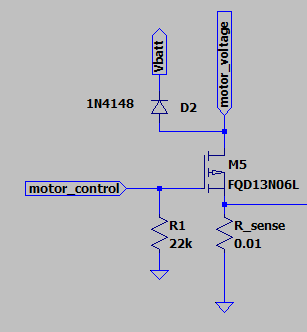
\includegraphics[width = 0.4\textwidth]{./Figures/Low_Switch_Cir.png}
\caption{Circuit diagram used for low side switching.}
\label{fig:low_switch_cir}
\end{figure}

\section{Current sensor Digital Wheel}
Since the the switching frequency is much larger than the \SI{1}{\kilo\hertz} filter requirement for the analogue current sensor the exact same circuit design will be used for the digital side as increasing the response time of the circuit will not meaningfully affect performance as you will have to wait for the analogue side. This also reduces design complexity and will allow for easier control of the car as the output from the current sensors will be the same for the same voltage. See Section:\ref{sec:current_sensor_design} for design specifics.

\clearpage
\section{Range sensor and PWM control}
\subsection{Range sensor}
The range sensor returns a PWM signal where the high time indicates how long it tool for the sonic signal to hit an object and return. Thus to calculate the range measured by the sensor the time the signal is high is measured using the pulseIn function which returns the time in microseconds. The range is  then calculated using the following formula:\\ $range = 340 \cdot \frac{HighTime}{2} \cdot 1E-6$\\ 
The 340 is used for the speed of sound and dividing the high time by 2 gets the time to the object. This gives a distance in micrometer thus multiply by 1E-6 in order to get the range in meters.
\subsection{PWM control}
In order to calculate the duty cycle for the PWM control the range measured by the range sensor is limited to a maximum of 1 meter and then used to scale the maximum duty cycle. The speed command is then mapped from its range to the range of the duty cycle and added to the scaled duty cycle and the maximum duty cycle is then subtracted. This procedure is illustrated in the following pseudo-code:\\
\begin{align*}
& DutyCycleLimit = Range \cdot MaxDutyCycle\\
& MappedRange = Range/MaxRange \cdot MaxDutyCycle\\
& ControlDutyCycle = DutyCycleLimit+MappedRange-MaxDutyCycle\\
\end{align*}

This emulates the circuit used to control the analogue wheel and will result in similar behaviour. The full software system can be seen in Figure:\ref{fig:dig_ctrl_flow}.

\begin{figure}[H]
\centering
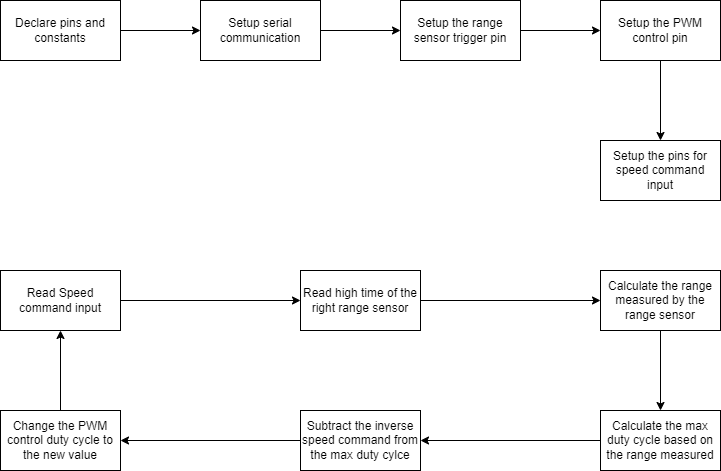
\includegraphics[width = 0.4\textwidth]{./Figures/Dig_Ctrl_Flow.png}
\caption{Flow diagram showing the software design.}
\label{fig:dig_ctrl_flow}
\end{figure}

\clearpage
\section{Battery Charger}

The battery charging circuit is shown in Figure:\ref{fig:bat_charg}. The only design for this section is selecting the mosfets M1 and M2 and designing the resistors R1-R5. Since M2 is being driven by the ESP it requires a low turn on voltage and thus the 2N7002 nmos will be used. M1 is used in a high side configuration and thus must be a pmos so the IRF9Z24N is used.\\

R3 and R5 are just used as pull up and pull down resistor respectively so any resistor value that is sufficiently large will work in order to limit current draw, \SI{220}{\kilo\ohm} resistors were chosen for this.\\

The voltage between the adjust pin and output pin on the voltage regulator is \SI{1.25}{\volt} \cite{LM317}. The following equations were used to calculate the required resistor values.
\begin{align*}
V_{out}-V_{adj}&=1.25\\
V_{adj}&=\frac{R_4}{R_2} \cdot \left(1.25-R_1 I_{out} \right)\\
\frac{R_4}{R_2} &= \frac{V_{out(max)}-V_{adj}}{V_{adj}}\\
V_1 &=V_{out}-I_{out}R_1\\
V_1 &=V_{bat}+V_{M1}+V_{D1}\\
R_1 &=\frac{V_{out}(@400mA)- V_1(@400mA)}{400mA}
\end{align*} 

These calculations result in R1 of \SI{0.45}{\ohm} and a R4:R2 ratio of 5:1.\\
R2 was chosen to be \SI{220}{\ohm} as this matches the recommended value in the datasheet \cite{LM317}.
 
\begin{figure}[H]
\centering
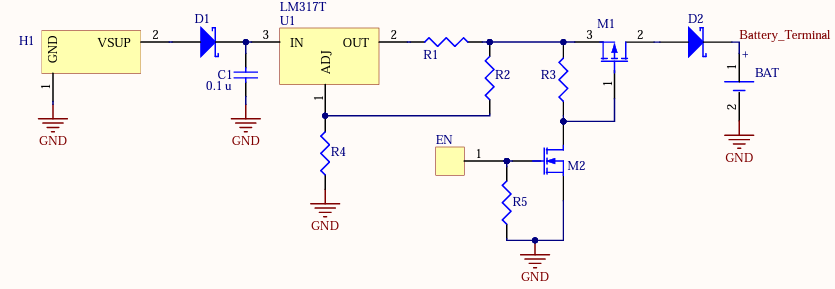
\includegraphics[width = 0.4\textwidth]{./Figures/Bat_Charg.png}
\caption{Battery charging circuit.}
\label{fig:bat_charg}
\end{figure}

\clearpage
\section{Voltage conditioning}

It was decided that the voltage regulator would convert a voltage between 5 and 7.6V to 0 to 3.3V. The upper limit of 7.6 was chosen inorder to protect the ESP that will be reading the voltage and thus no voltage divider circuit will be needed. Thus a simple difference amplifier will be used to subtract the 5V from the battery voltage and then correctly scale the signal into the correct range. The required gain was calculated as follows:
\begin{align*}
G = \frac{V_{out(max)}}{V_{bat(max)} - V_{offset}}
\end{align*}

This results in a gain of 1.27, a base resistance of \SI{120}{\kilo\ohm} was chosen. See Figure: \ref{fig:volt_cond} for the circuit diagram. R5 = R7 = \SI{120}{\kilo\ohm}  and R6 = R8 = 1.27 \SI{120}{\kilo\ohm}.

\begin{figure}[H]
\centering
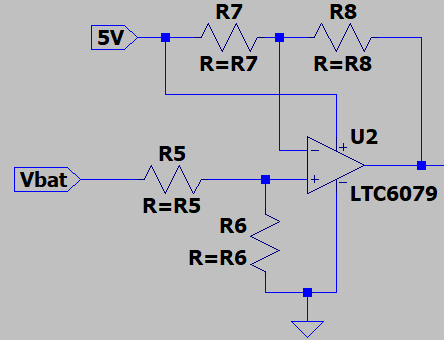
\includegraphics[width = 0.4\textwidth]{./Figures/Volt_Cond.png}
\caption{Voltage conditioning circuit.}
\label{fig:volt_cond}
\end{figure}


\clearpage
\section{Under-voltage protection}

The under voltage protection is implemented using a Schmitt Trigger circuit see Figure: \ref{fig:schmitt_trig} for the circuit diagram. Note R9 represents the motor load. The input to the Schmitt trigger will be the output from the voltage  conditioning circuit as this results in a larger range and means the circuit is less sensitive to component tolerances. The following equations were used to calculate the component values:
\begin{align*}
V_{out(high)} & = 5\\
V_{out(low)} & = 0\\
V_{in(high)} & = 1.5231\\
V_{in(low)} & = 1.2693\\
V_{offset} &=\frac{V_{in(low)} \cdot V_{out(high)}}{V_{out(high)} + V_{in(low)} - V_{in(high)}}\\
V_{offset} &=5 \cdot \frac{R_4}{R_3+R_4}\\
R_2 &= \frac{-V_{offset}}{V_{in(low)}-V_{offset}} \cdot R_1\\
\end{align*}

These calculations result in the following resistor values: R1 = \SI{3.3}{\kilo\ohm}, R2 = \SI{65}{\kilo\ohm}, R3 = \SI{120}{\kilo\ohm}, R4 = \SI{43.8}{\kilo\ohm}.

\begin{figure}[H]
\centering
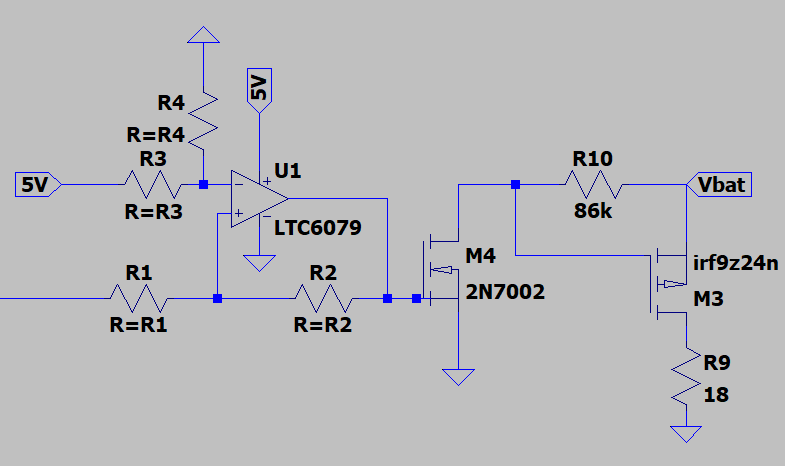
\includegraphics[width = 0.4\textwidth]{./Figures/Schmitt_Trig.png}
\caption{Under voltage protection circuit.}
\label{fig:schmitt_trig}
\end{figure}








